\documentclass[twoside]{book}

% Packages required by doxygen
\usepackage{fixltx2e}
\usepackage{calc}
\usepackage{doxygen}
\usepackage[export]{adjustbox} % also loads graphicx
\usepackage{graphicx}
\usepackage[utf8]{inputenc}
\usepackage{makeidx}
\usepackage{multicol}
\usepackage{multirow}
\PassOptionsToPackage{warn}{textcomp}
\usepackage{textcomp}
\usepackage[nointegrals]{wasysym}
\usepackage[table]{xcolor}

% Font selection
\usepackage[T1]{fontenc}
\usepackage[scaled=.90]{helvet}
\usepackage{courier}
\usepackage{amssymb}
\usepackage{sectsty}
\renewcommand{\familydefault}{\sfdefault}
\allsectionsfont{%
  \fontseries{bc}\selectfont%
  \color{darkgray}%
}
\renewcommand{\DoxyLabelFont}{%
  \fontseries{bc}\selectfont%
  \color{darkgray}%
}
\newcommand{\+}{\discretionary{\mbox{\scriptsize$\hookleftarrow$}}{}{}}

% Page & text layout
\usepackage{geometry}
\geometry{%
  a4paper,%
  top=2.5cm,%
  bottom=2.5cm,%
  left=2.5cm,%
  right=2.5cm%
}
\tolerance=750
\hfuzz=15pt
\hbadness=750
\setlength{\emergencystretch}{15pt}
\setlength{\parindent}{0cm}
\setlength{\parskip}{3ex plus 2ex minus 2ex}
\makeatletter
\renewcommand{\paragraph}{%
  \@startsection{paragraph}{4}{0ex}{-1.0ex}{1.0ex}{%
    \normalfont\normalsize\bfseries\SS@parafont%
  }%
}
\renewcommand{\subparagraph}{%
  \@startsection{subparagraph}{5}{0ex}{-1.0ex}{1.0ex}{%
    \normalfont\normalsize\bfseries\SS@subparafont%
  }%
}
\makeatother

% Headers & footers
\usepackage{fancyhdr}
\pagestyle{fancyplain}
\fancyhead[LE]{\fancyplain{}{\bfseries\thepage}}
\fancyhead[CE]{\fancyplain{}{}}
\fancyhead[RE]{\fancyplain{}{\bfseries\leftmark}}
\fancyhead[LO]{\fancyplain{}{\bfseries\rightmark}}
\fancyhead[CO]{\fancyplain{}{}}
\fancyhead[RO]{\fancyplain{}{\bfseries\thepage}}
\fancyfoot[LE]{\fancyplain{}{}}
\fancyfoot[CE]{\fancyplain{}{}}
\fancyfoot[RE]{\fancyplain{}{\bfseries\scriptsize Generated by Doxygen }}
\fancyfoot[LO]{\fancyplain{}{\bfseries\scriptsize Generated by Doxygen }}
\fancyfoot[CO]{\fancyplain{}{}}
\fancyfoot[RO]{\fancyplain{}{}}
\renewcommand{\footrulewidth}{0.4pt}
\renewcommand{\chaptermark}[1]{%
  \markboth{#1}{}%
}
\renewcommand{\sectionmark}[1]{%
  \markright{\thesection\ #1}%
}

% Indices & bibliography
\usepackage{natbib}
\usepackage[titles]{tocloft}
\setcounter{tocdepth}{3}
\setcounter{secnumdepth}{5}
\makeindex

% Hyperlinks (required, but should be loaded last)
\usepackage{ifpdf}
\ifpdf
  \usepackage[pdftex,pagebackref=true]{hyperref}
\else
  \usepackage[ps2pdf,pagebackref=true]{hyperref}
\fi
\hypersetup{%
  colorlinks=true,%
  linkcolor=blue,%
  citecolor=blue,%
  unicode%
}

% Custom commands
\newcommand{\clearemptydoublepage}{%
  \newpage{\pagestyle{empty}\cleardoublepage}%
}

\usepackage{caption}
\captionsetup{labelsep=space,justification=centering,font={bf},singlelinecheck=off,skip=4pt,position=top}

%===== C O N T E N T S =====

\begin{document}

% Titlepage & ToC
\hypersetup{pageanchor=false,
             bookmarksnumbered=true,
             pdfencoding=unicode
            }
\pagenumbering{roman}
\begin{titlepage}
\vspace*{7cm}
\begin{center}%
{\Large My Project }\\
\vspace*{1cm}
{\large Generated by Doxygen 1.8.11}\\
\end{center}
\end{titlepage}
\clearemptydoublepage
\tableofcontents
\clearemptydoublepage
\pagenumbering{arabic}
\hypersetup{pageanchor=true}

%--- Begin generated contents ---
\chapter{Hierarchical Index}
\section{Class Hierarchy}
This inheritance list is sorted roughly, but not completely, alphabetically\+:\begin{DoxyCompactList}
\item \contentsline{section}{Fruit}{\pageref{classFruit}}{}
\begin{DoxyCompactList}
\item \contentsline{section}{Apple}{\pageref{classApple}}{}
\item \contentsline{section}{Grape}{\pageref{classGrape}}{}
\item \contentsline{section}{Orange}{\pageref{classOrange}}{}
\end{DoxyCompactList}
\item \contentsline{section}{List}{\pageref{classList}}{}
\item \contentsline{section}{List\+:\+:Node}{\pageref{structList_1_1Node}}{}
\end{DoxyCompactList}

\chapter{Class Index}
\section{Class List}
Here are the classes, structs, unions and interfaces with brief descriptions\+:\begin{DoxyCompactList}
\item\contentsline{section}{\hyperlink{structnode}{node} }{\pageref{structnode}}{}
\item\contentsline{section}{\hyperlink{structnode1}{node1} }{\pageref{structnode1}}{}
\item\contentsline{section}{\hyperlink{structnode__info}{node\+\_\+info} }{\pageref{structnode__info}}{}
\end{DoxyCompactList}

\chapter{File Index}
\section{File List}
Here is a list of all files with brief descriptions\+:\begin{DoxyCompactList}
\item\contentsline{section}{\hyperlink{Lab1_8c}{Lab1.\+c} }{\pageref{Lab1_8c}}{}
\end{DoxyCompactList}

\chapter{Class Documentation}
\hypertarget{classDivingState}{}\section{Diving\+State Class Reference}
\label{classDivingState}\index{Diving\+State@{Diving\+State}}


Inheritance diagram for Diving\+State\+:
\nopagebreak
\begin{figure}[H]
\begin{center}
\leavevmode
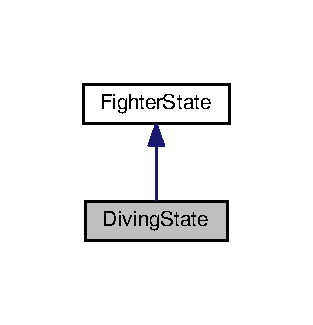
\includegraphics[width=150pt]{classDivingState__inherit__graph}
\end{center}
\end{figure}


Collaboration diagram for Diving\+State\+:
\nopagebreak
\begin{figure}[H]
\begin{center}
\leavevmode
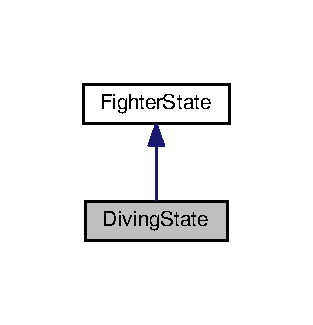
\includegraphics[width=150pt]{classDivingState__coll__graph}
\end{center}
\end{figure}
\subsection*{Public Member Functions}
\begin{DoxyCompactItemize}
\item 
virtual void \hyperlink{classDivingState_a22ddb04b1b75366cc8f9f5b017338498}{handle\+Input} (\hyperlink{classFighter}{Fighter} \&, \hyperlink{State_8cpp_a080a822f0093973313bd644e517a5090}{Input}) override
\item 
virtual void \hyperlink{classDivingState_a98ec5b0c6a09c934c0ab11694e8a6b4a}{update} (\hyperlink{classFighter}{Fighter} \&) override
\end{DoxyCompactItemize}
\subsection*{Additional Inherited Members}


\subsection{Member Function Documentation}
\index{Diving\+State@{Diving\+State}!handle\+Input@{handle\+Input}}
\index{handle\+Input@{handle\+Input}!Diving\+State@{Diving\+State}}
\subsubsection[{\texorpdfstring{handle\+Input(\+Fighter \&, Input) override}{handleInput(Fighter &, Input) override}}]{\setlength{\rightskip}{0pt plus 5cm}void Diving\+State\+::handle\+Input (
\begin{DoxyParamCaption}
\item[{{\bf Fighter} \&}]{fighter, }
\item[{{\bf Input}}]{}
\end{DoxyParamCaption}
)\hspace{0.3cm}{\ttfamily [override]}, {\ttfamily [virtual]}}\hypertarget{classDivingState_a22ddb04b1b75366cc8f9f5b017338498}{}\label{classDivingState_a22ddb04b1b75366cc8f9f5b017338498}


Implements \hyperlink{classFighterState_a84fcd7da4d232e79e1be9b32c0767861}{Fighter\+State}.


\begin{DoxyCode}
128                                                        \{
129     std::cout << \textcolor{stringliteral}{"Regardless of what the user input is, "} << fighter.\hyperlink{classFighter_aea4a9cf98a672b2305d1147885b91c34}{getName}() << \textcolor{stringliteral}{" lands from his
       dive and is now standing again."} << std::endl;
130     fighter.\hyperlink{classFighter_add08055f60abd6e9235291b653f65be5}{changeState} (\hyperlink{classFighterState_a050e9b5aff81843be5feea296a586889}{FighterState::standing});
131 \}
\end{DoxyCode}


Here is the call graph for this function\+:
\nopagebreak
\begin{figure}[H]
\begin{center}
\leavevmode
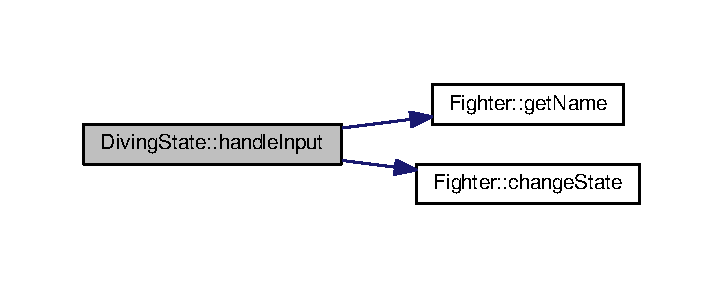
\includegraphics[width=347pt]{classDivingState_a22ddb04b1b75366cc8f9f5b017338498_cgraph}
\end{center}
\end{figure}


\index{Diving\+State@{Diving\+State}!update@{update}}
\index{update@{update}!Diving\+State@{Diving\+State}}
\subsubsection[{\texorpdfstring{update(\+Fighter \&) override}{update(Fighter &) override}}]{\setlength{\rightskip}{0pt plus 5cm}void Diving\+State\+::update (
\begin{DoxyParamCaption}
\item[{{\bf Fighter} \&}]{fighter}
\end{DoxyParamCaption}
)\hspace{0.3cm}{\ttfamily [override]}, {\ttfamily [virtual]}}\hypertarget{classDivingState_a98ec5b0c6a09c934c0ab11694e8a6b4a}{}\label{classDivingState_a98ec5b0c6a09c934c0ab11694e8a6b4a}


Implements \hyperlink{classFighterState_af022f76c6b1fe080047ded2280ec6f8f}{Fighter\+State}.


\begin{DoxyCode}
133                                           \{
134     fighter.\hyperlink{classFighter_aa9c08ec29097e326eab0ffd69db18b9c}{changeFatigueLevelBy}(2);
135 \}
\end{DoxyCode}


Here is the call graph for this function\+:
\nopagebreak
\begin{figure}[H]
\begin{center}
\leavevmode
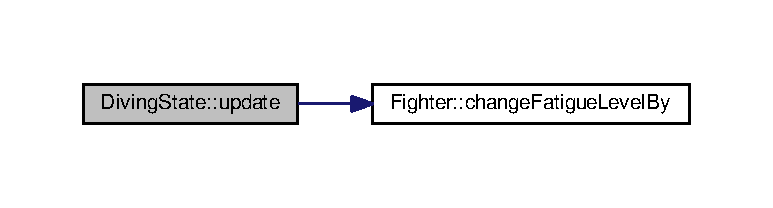
\includegraphics[width=350pt]{classDivingState_a98ec5b0c6a09c934c0ab11694e8a6b4a_cgraph}
\end{center}
\end{figure}




The documentation for this class was generated from the following file\+:\begin{DoxyCompactItemize}
\item 
\hyperlink{State_8cpp}{State.\+cpp}\end{DoxyCompactItemize}

\hypertarget{classDuckingState}{}\section{Ducking\+State Class Reference}
\label{classDuckingState}\index{Ducking\+State@{Ducking\+State}}


Inheritance diagram for Ducking\+State\+:
\nopagebreak
\begin{figure}[H]
\begin{center}
\leavevmode
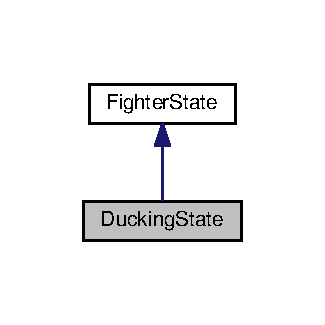
\includegraphics[width=156pt]{classDuckingState__inherit__graph}
\end{center}
\end{figure}


Collaboration diagram for Ducking\+State\+:
\nopagebreak
\begin{figure}[H]
\begin{center}
\leavevmode
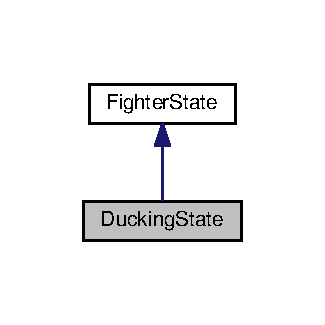
\includegraphics[width=156pt]{classDuckingState__coll__graph}
\end{center}
\end{figure}
\subsection*{Public Member Functions}
\begin{DoxyCompactItemize}
\item 
\hyperlink{classDuckingState_a62f30e2eac4a71c01d3870cf63899725}{Ducking\+State} ()
\item 
virtual void \hyperlink{classDuckingState_a233ad7f72fa53e13a28a090d097a845b}{handle\+Input} (\hyperlink{classFighter}{Fighter} \&, \hyperlink{State_8cpp_a080a822f0093973313bd644e517a5090}{Input}) override
\item 
virtual void \hyperlink{classDuckingState_a634612b9f2d152c8805366541a775504}{update} (\hyperlink{classFighter}{Fighter} \&) override
\end{DoxyCompactItemize}
\subsection*{Private Attributes}
\begin{DoxyCompactItemize}
\item 
int \hyperlink{classDuckingState_abb35456dc6b1c0fc15b2238ceafbb817}{charging\+Time}
\end{DoxyCompactItemize}
\subsection*{Static Private Attributes}
\begin{DoxyCompactItemize}
\item 
static const int \hyperlink{classDuckingState_a1af568ef268261b3be1773b23d343b4a}{Full\+Rest\+Time} = 5
\end{DoxyCompactItemize}
\subsection*{Additional Inherited Members}


\subsection{Constructor \& Destructor Documentation}
\index{Ducking\+State@{Ducking\+State}!Ducking\+State@{Ducking\+State}}
\index{Ducking\+State@{Ducking\+State}!Ducking\+State@{Ducking\+State}}
\subsubsection[{\texorpdfstring{Ducking\+State()}{DuckingState()}}]{\setlength{\rightskip}{0pt plus 5cm}Ducking\+State\+::\+Ducking\+State (
\begin{DoxyParamCaption}
{}
\end{DoxyParamCaption}
)\hspace{0.3cm}{\ttfamily [inline]}}\hypertarget{classDuckingState_a62f30e2eac4a71c01d3870cf63899725}{}\label{classDuckingState_a62f30e2eac4a71c01d3870cf63899725}

\begin{DoxyCode}
26 : \hyperlink{classDuckingState_abb35456dc6b1c0fc15b2238ceafbb817}{chargingTime}(0) \{\}
\end{DoxyCode}


Here is the call graph for this function\+:
\nopagebreak
\begin{figure}[H]
\begin{center}
\leavevmode
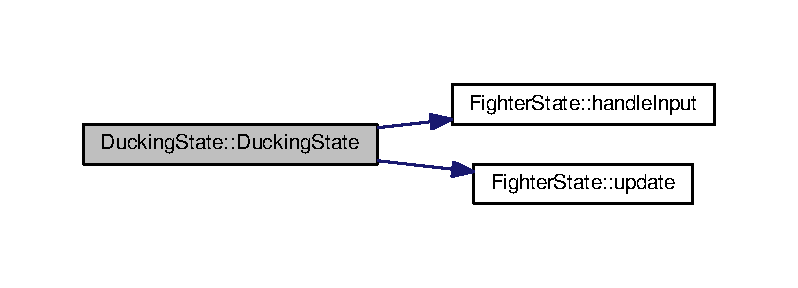
\includegraphics[width=350pt]{classDuckingState_a62f30e2eac4a71c01d3870cf63899725_cgraph}
\end{center}
\end{figure}




\subsection{Member Function Documentation}
\index{Ducking\+State@{Ducking\+State}!handle\+Input@{handle\+Input}}
\index{handle\+Input@{handle\+Input}!Ducking\+State@{Ducking\+State}}
\subsubsection[{\texorpdfstring{handle\+Input(\+Fighter \&, Input) override}{handleInput(Fighter &, Input) override}}]{\setlength{\rightskip}{0pt plus 5cm}void Ducking\+State\+::handle\+Input (
\begin{DoxyParamCaption}
\item[{{\bf Fighter} \&}]{fighter, }
\item[{{\bf Input}}]{input}
\end{DoxyParamCaption}
)\hspace{0.3cm}{\ttfamily [override]}, {\ttfamily [virtual]}}\hypertarget{classDuckingState_a233ad7f72fa53e13a28a090d097a845b}{}\label{classDuckingState_a233ad7f72fa53e13a28a090d097a845b}


Implements \hyperlink{classFighterState_a84fcd7da4d232e79e1be9b32c0767861}{Fighter\+State}.


\begin{DoxyCode}
90                                                               \{
91     \textcolor{keywordflow}{switch} (input) \{
92         \textcolor{keywordflow}{case} \hyperlink{State_8cpp_a080a822f0093973313bd644e517a5090a4e0f05b608ae82cd3d38087399f6962a}{STAND\_UP}:  fighter.\hyperlink{classFighter_add08055f60abd6e9235291b653f65be5}{changeState} (
      \hyperlink{classFighterState_a050e9b5aff81843be5feea296a586889}{FighterState::standing});  \textcolor{keywordflow}{return} fighter.\hyperlink{classFighter_a6f54ee51d7ca6b3baa60dd19bb4546c5}{standsUp}();
93         \textcolor{keywordflow}{case} \hyperlink{State_8cpp_a080a822f0093973313bd644e517a5090af82233b8404f602e50c8fb3fff20db8d}{DUCK\_DOWN}:
94             std::cout << fighter.\hyperlink{classFighter_aea4a9cf98a672b2305d1147885b91c34}{getName}() << \textcolor{stringliteral}{" remains in ducking position, "};
95             \textcolor{keywordflow}{if} (\hyperlink{classDuckingState_abb35456dc6b1c0fc15b2238ceafbb817}{chargingTime} < \hyperlink{classDuckingState_a1af568ef268261b3be1773b23d343b4a}{FullRestTime}) std::cout << \textcolor{stringliteral}{"recovering in the
       meantime."} << std::endl;
96             \textcolor{keywordflow}{else} std::cout << \textcolor{stringliteral}{"fully recovered."} << std::endl;
97             \textcolor{keywordflow}{return} \hyperlink{classDuckingState_a634612b9f2d152c8805366541a775504}{update} (fighter);
98         \textcolor{keywordflow}{default}:
99             std::cout << \textcolor{stringliteral}{"One cannot do that while ducking.  "} << fighter.
      \hyperlink{classFighter_aea4a9cf98a672b2305d1147885b91c34}{getName}() << \textcolor{stringliteral}{" remains in ducking position by default."} << std::endl;
100             \hyperlink{classDuckingState_a634612b9f2d152c8805366541a775504}{update} (fighter);
101     \}
102 \}
\end{DoxyCode}


Here is the call graph for this function\+:
\nopagebreak
\begin{figure}[H]
\begin{center}
\leavevmode
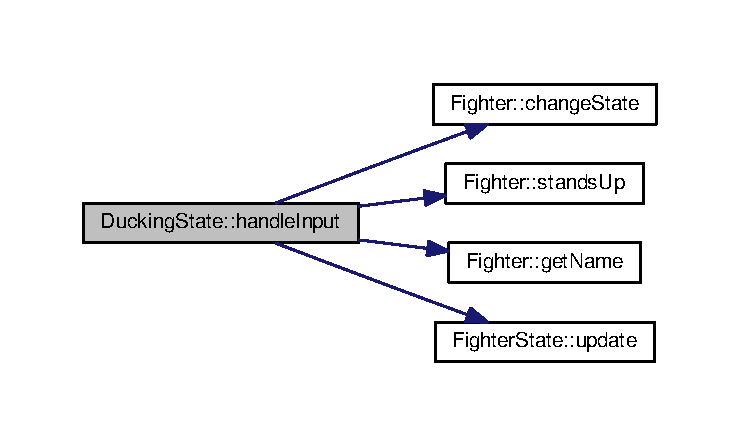
\includegraphics[width=350pt]{classDuckingState_a233ad7f72fa53e13a28a090d097a845b_cgraph}
\end{center}
\end{figure}


\index{Ducking\+State@{Ducking\+State}!update@{update}}
\index{update@{update}!Ducking\+State@{Ducking\+State}}
\subsubsection[{\texorpdfstring{update(\+Fighter \&) override}{update(Fighter &) override}}]{\setlength{\rightskip}{0pt plus 5cm}void Ducking\+State\+::update (
\begin{DoxyParamCaption}
\item[{{\bf Fighter} \&}]{fighter}
\end{DoxyParamCaption}
)\hspace{0.3cm}{\ttfamily [override]}, {\ttfamily [virtual]}}\hypertarget{classDuckingState_a634612b9f2d152c8805366541a775504}{}\label{classDuckingState_a634612b9f2d152c8805366541a775504}


Implements \hyperlink{classFighterState_af022f76c6b1fe080047ded2280ec6f8f}{Fighter\+State}.


\begin{DoxyCode}
104                                            \{
105     \hyperlink{classDuckingState_abb35456dc6b1c0fc15b2238ceafbb817}{chargingTime}++;
106     std::cout << \textcolor{stringliteral}{"Charging time = "} << \hyperlink{classDuckingState_abb35456dc6b1c0fc15b2238ceafbb817}{chargingTime} << \textcolor{stringliteral}{"."} << std::endl;
107     \textcolor{keywordflow}{if} (fighter.\hyperlink{classFighter_a1bc4025d988b66dfceaf0005e74f34ff}{getFatigueLevel}() > 0)
108         fighter.\hyperlink{classFighter_aa9c08ec29097e326eab0ffd69db18b9c}{changeFatigueLevelBy}(-1);
109     \textcolor{keywordflow}{if} (\hyperlink{classDuckingState_abb35456dc6b1c0fc15b2238ceafbb817}{chargingTime} >= \hyperlink{classDuckingState_a1af568ef268261b3be1773b23d343b4a}{FullRestTime} && fighter.
      \hyperlink{classFighter_a1bc4025d988b66dfceaf0005e74f34ff}{getFatigueLevel}() <= 3)
110         fighter.\hyperlink{classFighter_ae54fd861131ec55b366a9163a35d9606}{feelsStrong}();
111 \}
\end{DoxyCode}


Here is the call graph for this function\+:
\nopagebreak
\begin{figure}[H]
\begin{center}
\leavevmode
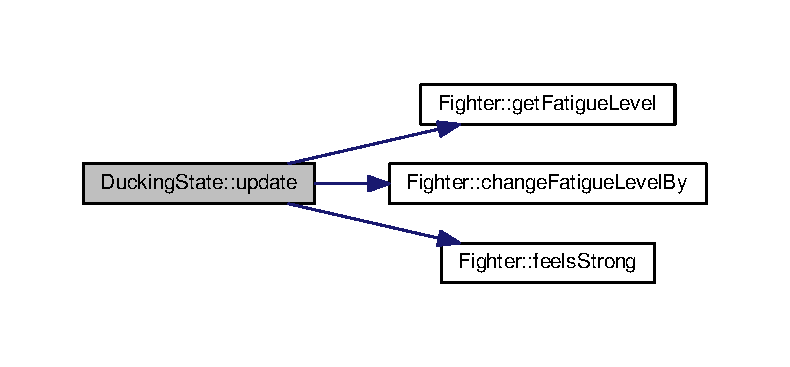
\includegraphics[width=350pt]{classDuckingState_a634612b9f2d152c8805366541a775504_cgraph}
\end{center}
\end{figure}




\subsection{Member Data Documentation}
\index{Ducking\+State@{Ducking\+State}!charging\+Time@{charging\+Time}}
\index{charging\+Time@{charging\+Time}!Ducking\+State@{Ducking\+State}}
\subsubsection[{\texorpdfstring{charging\+Time}{chargingTime}}]{\setlength{\rightskip}{0pt plus 5cm}int Ducking\+State\+::charging\+Time\hspace{0.3cm}{\ttfamily [private]}}\hypertarget{classDuckingState_abb35456dc6b1c0fc15b2238ceafbb817}{}\label{classDuckingState_abb35456dc6b1c0fc15b2238ceafbb817}
\index{Ducking\+State@{Ducking\+State}!Full\+Rest\+Time@{Full\+Rest\+Time}}
\index{Full\+Rest\+Time@{Full\+Rest\+Time}!Ducking\+State@{Ducking\+State}}
\subsubsection[{\texorpdfstring{Full\+Rest\+Time}{FullRestTime}}]{\setlength{\rightskip}{0pt plus 5cm}const int Ducking\+State\+::\+Full\+Rest\+Time = 5\hspace{0.3cm}{\ttfamily [static]}, {\ttfamily [private]}}\hypertarget{classDuckingState_a1af568ef268261b3be1773b23d343b4a}{}\label{classDuckingState_a1af568ef268261b3be1773b23d343b4a}


The documentation for this class was generated from the following file\+:\begin{DoxyCompactItemize}
\item 
\hyperlink{State_8cpp}{State.\+cpp}\end{DoxyCompactItemize}

\hypertarget{classFighter}{}\section{Fighter Class Reference}
\label{classFighter}\index{Fighter@{Fighter}}
\subsection*{Public Member Functions}
\begin{DoxyCompactItemize}
\item 
\hyperlink{classFighter_a2c8f42ee30394dc361c659c26666b0a5}{Fighter} (const std\+::string \&new\+Name)
\item 
std\+::string \hyperlink{classFighter_aea4a9cf98a672b2305d1147885b91c34}{get\+Name} () const 
\item 
int \hyperlink{classFighter_a1bc4025d988b66dfceaf0005e74f34ff}{get\+Fatigue\+Level} () const 
\item 
virtual void \hyperlink{classFighter_a178751f22e18d2e5cb02a05a766f6b24}{handle\+Input} (\hyperlink{State_8cpp_a080a822f0093973313bd644e517a5090}{Input} input)
\item 
void \hyperlink{classFighter_add08055f60abd6e9235291b653f65be5}{change\+State} (std\+::shared\+\_\+ptr$<$ \hyperlink{classFighterState}{Fighter\+State} $>$ new\+State)
\item 
void \hyperlink{classFighter_a6f54ee51d7ca6b3baa60dd19bb4546c5}{stands\+Up} ()
\item 
void \hyperlink{classFighter_afff11a1b3dacee662cb3fbe35f54df17}{ducks\+Down} ()
\item 
void \hyperlink{classFighter_a32a4250077afba9b3629a8f553dd8776}{jumps} ()
\item 
void \hyperlink{classFighter_a56cef6bffcdf9775f9d924cd213ed704}{dives} ()
\item 
void \hyperlink{classFighter_ae54fd861131ec55b366a9163a35d9606}{feels\+Strong} ()
\item 
void \hyperlink{classFighter_aa9c08ec29097e326eab0ffd69db18b9c}{change\+Fatigue\+Level\+By} (int change)
\end{DoxyCompactItemize}
\subsection*{Private Member Functions}
\begin{DoxyCompactItemize}
\item 
virtual void \hyperlink{classFighter_a0bd51ab4d6d20942b9f2fca23e1e7e4b}{update\+With\+New\+State} ()
\end{DoxyCompactItemize}
\subsection*{Private Attributes}
\begin{DoxyCompactItemize}
\item 
std\+::string \hyperlink{classFighter_a1b57178f9d5293da5f9d3d28cab097dc}{name}
\item 
std\+::shared\+\_\+ptr$<$ \hyperlink{classFighterState}{Fighter\+State} $>$ \hyperlink{classFighter_a3221c5b17cd0e0ffcb4333bbd3fca734}{state}
\item 
int \hyperlink{classFighter_aa54661200c35e46a969c4efd97e84784}{fatigue\+Level} = std\+::rand() \% 10
\end{DoxyCompactItemize}


\subsection{Constructor \& Destructor Documentation}
\index{Fighter@{Fighter}!Fighter@{Fighter}}
\index{Fighter@{Fighter}!Fighter@{Fighter}}
\subsubsection[{\texorpdfstring{Fighter(const std\+::string \&new\+Name)}{Fighter(const std::string &newName)}}]{\setlength{\rightskip}{0pt plus 5cm}Fighter\+::\+Fighter (
\begin{DoxyParamCaption}
\item[{const std\+::string \&}]{new\+Name}
\end{DoxyParamCaption}
)\hspace{0.3cm}{\ttfamily [inline]}}\hypertarget{classFighter_a2c8f42ee30394dc361c659c26666b0a5}{}\label{classFighter_a2c8f42ee30394dc361c659c26666b0a5}

\begin{DoxyCode}
61 : \hyperlink{classFighter_a1b57178f9d5293da5f9d3d28cab097dc}{name} (newName), \hyperlink{classFighter_a3221c5b17cd0e0ffcb4333bbd3fca734}{state} (\hyperlink{classFighterState_a050e9b5aff81843be5feea296a586889}{FighterState::standing}) \{\}
\end{DoxyCode}


\subsection{Member Function Documentation}
\index{Fighter@{Fighter}!change\+Fatigue\+Level\+By@{change\+Fatigue\+Level\+By}}
\index{change\+Fatigue\+Level\+By@{change\+Fatigue\+Level\+By}!Fighter@{Fighter}}
\subsubsection[{\texorpdfstring{change\+Fatigue\+Level\+By(int change)}{changeFatigueLevelBy(int change)}}]{\setlength{\rightskip}{0pt plus 5cm}void Fighter\+::change\+Fatigue\+Level\+By (
\begin{DoxyParamCaption}
\item[{int}]{change}
\end{DoxyParamCaption}
)\hspace{0.3cm}{\ttfamily [inline]}}\hypertarget{classFighter_aa9c08ec29097e326eab0ffd69db18b9c}{}\label{classFighter_aa9c08ec29097e326eab0ffd69db18b9c}

\begin{DoxyCode}
71 \{\hyperlink{classFighter_aa54661200c35e46a969c4efd97e84784}{fatigueLevel} += change;  std::cout << \textcolor{stringliteral}{"fatigueLevel = "} << 
      \hyperlink{classFighter_aa54661200c35e46a969c4efd97e84784}{fatigueLevel} << std::endl;\}
\end{DoxyCode}
\index{Fighter@{Fighter}!change\+State@{change\+State}}
\index{change\+State@{change\+State}!Fighter@{Fighter}}
\subsubsection[{\texorpdfstring{change\+State(std\+::shared\+\_\+ptr$<$ Fighter\+State $>$ new\+State)}{changeState(std::shared_ptr< FighterState > newState)}}]{\setlength{\rightskip}{0pt plus 5cm}void Fighter\+::change\+State (
\begin{DoxyParamCaption}
\item[{std\+::shared\+\_\+ptr$<$ {\bf Fighter\+State} $>$}]{new\+State}
\end{DoxyParamCaption}
)\hspace{0.3cm}{\ttfamily [inline]}}\hypertarget{classFighter_add08055f60abd6e9235291b653f65be5}{}\label{classFighter_add08055f60abd6e9235291b653f65be5}

\begin{DoxyCode}
65 \{\hyperlink{classFighter_a3221c5b17cd0e0ffcb4333bbd3fca734}{state} = newState;  \hyperlink{classFighter_a0bd51ab4d6d20942b9f2fca23e1e7e4b}{updateWithNewState}();\}
\end{DoxyCode}
\index{Fighter@{Fighter}!dives@{dives}}
\index{dives@{dives}!Fighter@{Fighter}}
\subsubsection[{\texorpdfstring{dives()}{dives()}}]{\setlength{\rightskip}{0pt plus 5cm}void Fighter\+::dives (
\begin{DoxyParamCaption}
{}
\end{DoxyParamCaption}
)\hspace{0.3cm}{\ttfamily [inline]}}\hypertarget{classFighter_a56cef6bffcdf9775f9d924cd213ed704}{}\label{classFighter_a56cef6bffcdf9775f9d924cd213ed704}

\begin{DoxyCode}
69 \{std::cout << \hyperlink{classFighter_aea4a9cf98a672b2305d1147885b91c34}{getName}() << \textcolor{stringliteral}{" makes a dive attack in the middle of the jump!"} << std::endl;\}
\end{DoxyCode}
\index{Fighter@{Fighter}!ducks\+Down@{ducks\+Down}}
\index{ducks\+Down@{ducks\+Down}!Fighter@{Fighter}}
\subsubsection[{\texorpdfstring{ducks\+Down()}{ducksDown()}}]{\setlength{\rightskip}{0pt plus 5cm}void Fighter\+::ducks\+Down (
\begin{DoxyParamCaption}
{}
\end{DoxyParamCaption}
)\hspace{0.3cm}{\ttfamily [inline]}}\hypertarget{classFighter_afff11a1b3dacee662cb3fbe35f54df17}{}\label{classFighter_afff11a1b3dacee662cb3fbe35f54df17}

\begin{DoxyCode}
67 \{std::cout << \hyperlink{classFighter_aea4a9cf98a672b2305d1147885b91c34}{getName}() << \textcolor{stringliteral}{" ducks down."} << std::endl;\}
\end{DoxyCode}
\index{Fighter@{Fighter}!feels\+Strong@{feels\+Strong}}
\index{feels\+Strong@{feels\+Strong}!Fighter@{Fighter}}
\subsubsection[{\texorpdfstring{feels\+Strong()}{feelsStrong()}}]{\setlength{\rightskip}{0pt plus 5cm}void Fighter\+::feels\+Strong (
\begin{DoxyParamCaption}
{}
\end{DoxyParamCaption}
)\hspace{0.3cm}{\ttfamily [inline]}}\hypertarget{classFighter_ae54fd861131ec55b366a9163a35d9606}{}\label{classFighter_ae54fd861131ec55b366a9163a35d9606}

\begin{DoxyCode}
70 \{std::cout << \hyperlink{classFighter_aea4a9cf98a672b2305d1147885b91c34}{getName}() << \textcolor{stringliteral}{" feels strong!"} << std::endl;\}
\end{DoxyCode}
\index{Fighter@{Fighter}!get\+Fatigue\+Level@{get\+Fatigue\+Level}}
\index{get\+Fatigue\+Level@{get\+Fatigue\+Level}!Fighter@{Fighter}}
\subsubsection[{\texorpdfstring{get\+Fatigue\+Level() const }{getFatigueLevel() const }}]{\setlength{\rightskip}{0pt plus 5cm}int Fighter\+::get\+Fatigue\+Level (
\begin{DoxyParamCaption}
{}
\end{DoxyParamCaption}
) const\hspace{0.3cm}{\ttfamily [inline]}}\hypertarget{classFighter_a1bc4025d988b66dfceaf0005e74f34ff}{}\label{classFighter_a1bc4025d988b66dfceaf0005e74f34ff}

\begin{DoxyCode}
63 \{\textcolor{keywordflow}{return} \hyperlink{classFighter_aa54661200c35e46a969c4efd97e84784}{fatigueLevel};\}
\end{DoxyCode}
\index{Fighter@{Fighter}!get\+Name@{get\+Name}}
\index{get\+Name@{get\+Name}!Fighter@{Fighter}}
\subsubsection[{\texorpdfstring{get\+Name() const }{getName() const }}]{\setlength{\rightskip}{0pt plus 5cm}std\+::string Fighter\+::get\+Name (
\begin{DoxyParamCaption}
{}
\end{DoxyParamCaption}
) const\hspace{0.3cm}{\ttfamily [inline]}}\hypertarget{classFighter_aea4a9cf98a672b2305d1147885b91c34}{}\label{classFighter_aea4a9cf98a672b2305d1147885b91c34}

\begin{DoxyCode}
62 \{\textcolor{keywordflow}{return} \hyperlink{classFighter_a1b57178f9d5293da5f9d3d28cab097dc}{name};\}
\end{DoxyCode}
\index{Fighter@{Fighter}!handle\+Input@{handle\+Input}}
\index{handle\+Input@{handle\+Input}!Fighter@{Fighter}}
\subsubsection[{\texorpdfstring{handle\+Input(\+Input input)}{handleInput(Input input)}}]{\setlength{\rightskip}{0pt plus 5cm}virtual void Fighter\+::handle\+Input (
\begin{DoxyParamCaption}
\item[{{\bf Input}}]{input}
\end{DoxyParamCaption}
)\hspace{0.3cm}{\ttfamily [inline]}, {\ttfamily [virtual]}}\hypertarget{classFighter_a178751f22e18d2e5cb02a05a766f6b24}{}\label{classFighter_a178751f22e18d2e5cb02a05a766f6b24}

\begin{DoxyCode}
64 \{\hyperlink{classFighter_a3221c5b17cd0e0ffcb4333bbd3fca734}{state}->handleInput (*\textcolor{keyword}{this}, input);\}  \textcolor{comment}{// delegate input handling to 'state'.}
\end{DoxyCode}
\index{Fighter@{Fighter}!jumps@{jumps}}
\index{jumps@{jumps}!Fighter@{Fighter}}
\subsubsection[{\texorpdfstring{jumps()}{jumps()}}]{\setlength{\rightskip}{0pt plus 5cm}void Fighter\+::jumps (
\begin{DoxyParamCaption}
{}
\end{DoxyParamCaption}
)\hspace{0.3cm}{\ttfamily [inline]}}\hypertarget{classFighter_a32a4250077afba9b3629a8f553dd8776}{}\label{classFighter_a32a4250077afba9b3629a8f553dd8776}

\begin{DoxyCode}
68 \{std::cout << \hyperlink{classFighter_aea4a9cf98a672b2305d1147885b91c34}{getName}() << \textcolor{stringliteral}{" jumps into the air."} << std::endl;\}
\end{DoxyCode}
\index{Fighter@{Fighter}!stands\+Up@{stands\+Up}}
\index{stands\+Up@{stands\+Up}!Fighter@{Fighter}}
\subsubsection[{\texorpdfstring{stands\+Up()}{standsUp()}}]{\setlength{\rightskip}{0pt plus 5cm}void Fighter\+::stands\+Up (
\begin{DoxyParamCaption}
{}
\end{DoxyParamCaption}
)\hspace{0.3cm}{\ttfamily [inline]}}\hypertarget{classFighter_a6f54ee51d7ca6b3baa60dd19bb4546c5}{}\label{classFighter_a6f54ee51d7ca6b3baa60dd19bb4546c5}

\begin{DoxyCode}
66 \{std::cout << \hyperlink{classFighter_aea4a9cf98a672b2305d1147885b91c34}{getName}() << \textcolor{stringliteral}{" stands up."} << std::endl;\}
\end{DoxyCode}
\index{Fighter@{Fighter}!update\+With\+New\+State@{update\+With\+New\+State}}
\index{update\+With\+New\+State@{update\+With\+New\+State}!Fighter@{Fighter}}
\subsubsection[{\texorpdfstring{update\+With\+New\+State()}{updateWithNewState()}}]{\setlength{\rightskip}{0pt plus 5cm}virtual void Fighter\+::update\+With\+New\+State (
\begin{DoxyParamCaption}
{}
\end{DoxyParamCaption}
)\hspace{0.3cm}{\ttfamily [inline]}, {\ttfamily [private]}, {\ttfamily [virtual]}}\hypertarget{classFighter_a0bd51ab4d6d20942b9f2fca23e1e7e4b}{}\label{classFighter_a0bd51ab4d6d20942b9f2fca23e1e7e4b}

\begin{DoxyCode}
73 \{\hyperlink{classFighter_a3221c5b17cd0e0ffcb4333bbd3fca734}{state}->update(*\textcolor{keyword}{this});\}  \textcolor{comment}{// delegate updating to 'state'}
\end{DoxyCode}


\subsection{Member Data Documentation}
\index{Fighter@{Fighter}!fatigue\+Level@{fatigue\+Level}}
\index{fatigue\+Level@{fatigue\+Level}!Fighter@{Fighter}}
\subsubsection[{\texorpdfstring{fatigue\+Level}{fatigueLevel}}]{\setlength{\rightskip}{0pt plus 5cm}int Fighter\+::fatigue\+Level = std\+::rand() \% 10\hspace{0.3cm}{\ttfamily [private]}}\hypertarget{classFighter_aa54661200c35e46a969c4efd97e84784}{}\label{classFighter_aa54661200c35e46a969c4efd97e84784}
\index{Fighter@{Fighter}!name@{name}}
\index{name@{name}!Fighter@{Fighter}}
\subsubsection[{\texorpdfstring{name}{name}}]{\setlength{\rightskip}{0pt plus 5cm}std\+::string Fighter\+::name\hspace{0.3cm}{\ttfamily [private]}}\hypertarget{classFighter_a1b57178f9d5293da5f9d3d28cab097dc}{}\label{classFighter_a1b57178f9d5293da5f9d3d28cab097dc}
\index{Fighter@{Fighter}!state@{state}}
\index{state@{state}!Fighter@{Fighter}}
\subsubsection[{\texorpdfstring{state}{state}}]{\setlength{\rightskip}{0pt plus 5cm}std\+::shared\+\_\+ptr$<${\bf Fighter\+State}$>$ Fighter\+::state\hspace{0.3cm}{\ttfamily [private]}}\hypertarget{classFighter_a3221c5b17cd0e0ffcb4333bbd3fca734}{}\label{classFighter_a3221c5b17cd0e0ffcb4333bbd3fca734}


The documentation for this class was generated from the following file\+:\begin{DoxyCompactItemize}
\item 
\hyperlink{State_8cpp}{State.\+cpp}\end{DoxyCompactItemize}

\hypertarget{classFighterState}{}\section{Fighter\+State Class Reference}
\label{classFighterState}\index{Fighter\+State@{Fighter\+State}}


Inheritance diagram for Fighter\+State\+:
\nopagebreak
\begin{figure}[H]
\begin{center}
\leavevmode
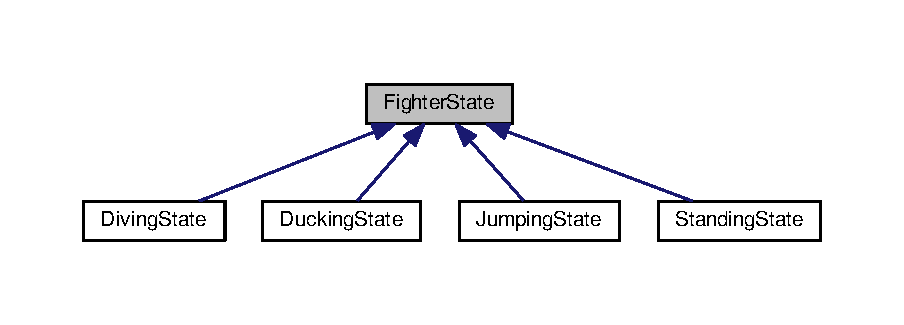
\includegraphics[width=350pt]{classFighterState__inherit__graph}
\end{center}
\end{figure}
\subsection*{Public Member Functions}
\begin{DoxyCompactItemize}
\item 
virtual \hyperlink{classFighterState_a5ee5999d79f6a7e8cdf386cbf05fb941}{$\sim$\+Fighter\+State} ()=default
\item 
virtual void \hyperlink{classFighterState_a84fcd7da4d232e79e1be9b32c0767861}{handle\+Input} (\hyperlink{classFighter}{Fighter} \&, \hyperlink{State_8cpp_a080a822f0093973313bd644e517a5090}{Input})=0
\item 
virtual void \hyperlink{classFighterState_af022f76c6b1fe080047ded2280ec6f8f}{update} (\hyperlink{classFighter}{Fighter} \&)=0
\end{DoxyCompactItemize}
\subsection*{Static Public Attributes}
\begin{DoxyCompactItemize}
\item 
static std\+::shared\+\_\+ptr$<$ \hyperlink{classStandingState}{Standing\+State} $>$ \hyperlink{classFighterState_a050e9b5aff81843be5feea296a586889}{standing}
\item 
static std\+::shared\+\_\+ptr$<$ \hyperlink{classDivingState}{Diving\+State} $>$ \hyperlink{classFighterState_ad4f8371e5a2d9e5b165d5c41072eb6d9}{diving}
\end{DoxyCompactItemize}


\subsection{Constructor \& Destructor Documentation}
\index{Fighter\+State@{Fighter\+State}!````~Fighter\+State@{$\sim$\+Fighter\+State}}
\index{````~Fighter\+State@{$\sim$\+Fighter\+State}!Fighter\+State@{Fighter\+State}}
\subsubsection[{\texorpdfstring{$\sim$\+Fighter\+State()=default}{~FighterState()=default}}]{\setlength{\rightskip}{0pt plus 5cm}virtual Fighter\+State\+::$\sim$\+Fighter\+State (
\begin{DoxyParamCaption}
{}
\end{DoxyParamCaption}
)\hspace{0.3cm}{\ttfamily [virtual]}, {\ttfamily [default]}}\hypertarget{classFighterState_a5ee5999d79f6a7e8cdf386cbf05fb941}{}\label{classFighterState_a5ee5999d79f6a7e8cdf386cbf05fb941}


\subsection{Member Function Documentation}
\index{Fighter\+State@{Fighter\+State}!handle\+Input@{handle\+Input}}
\index{handle\+Input@{handle\+Input}!Fighter\+State@{Fighter\+State}}
\subsubsection[{\texorpdfstring{handle\+Input(\+Fighter \&, Input)=0}{handleInput(Fighter &, Input)=0}}]{\setlength{\rightskip}{0pt plus 5cm}virtual void Fighter\+State\+::handle\+Input (
\begin{DoxyParamCaption}
\item[{{\bf Fighter} \&}]{, }
\item[{{\bf Input}}]{}
\end{DoxyParamCaption}
)\hspace{0.3cm}{\ttfamily [pure virtual]}}\hypertarget{classFighterState_a84fcd7da4d232e79e1be9b32c0767861}{}\label{classFighterState_a84fcd7da4d232e79e1be9b32c0767861}


Implemented in \hyperlink{classDivingState_a22ddb04b1b75366cc8f9f5b017338498}{Diving\+State}, \hyperlink{classJumpingState_a40be6d03f207fc425dfe2b1395fd4edb}{Jumping\+State}, \hyperlink{classStandingState_a63e99bb4fb71ef88ba573ad902337e7c}{Standing\+State}, and \hyperlink{classDuckingState_a233ad7f72fa53e13a28a090d097a845b}{Ducking\+State}.

\index{Fighter\+State@{Fighter\+State}!update@{update}}
\index{update@{update}!Fighter\+State@{Fighter\+State}}
\subsubsection[{\texorpdfstring{update(\+Fighter \&)=0}{update(Fighter &)=0}}]{\setlength{\rightskip}{0pt plus 5cm}virtual void Fighter\+State\+::update (
\begin{DoxyParamCaption}
\item[{{\bf Fighter} \&}]{}
\end{DoxyParamCaption}
)\hspace{0.3cm}{\ttfamily [pure virtual]}}\hypertarget{classFighterState_af022f76c6b1fe080047ded2280ec6f8f}{}\label{classFighterState_af022f76c6b1fe080047ded2280ec6f8f}


Implemented in \hyperlink{classDivingState_a98ec5b0c6a09c934c0ab11694e8a6b4a}{Diving\+State}, \hyperlink{classJumpingState_aef36270d1d3aec51bdf4770e9ad571c8}{Jumping\+State}, \hyperlink{classStandingState_a3a99901a53764049b39df5b8f016fb66}{Standing\+State}, and \hyperlink{classDuckingState_a634612b9f2d152c8805366541a775504}{Ducking\+State}.



\subsection{Member Data Documentation}
\index{Fighter\+State@{Fighter\+State}!diving@{diving}}
\index{diving@{diving}!Fighter\+State@{Fighter\+State}}
\subsubsection[{\texorpdfstring{diving}{diving}}]{\setlength{\rightskip}{0pt plus 5cm}std\+::shared\+\_\+ptr$<$ {\bf Diving\+State} $>$ Fighter\+State\+::diving\hspace{0.3cm}{\ttfamily [static]}}\hypertarget{classFighterState_ad4f8371e5a2d9e5b165d5c41072eb6d9}{}\label{classFighterState_ad4f8371e5a2d9e5b165d5c41072eb6d9}
\index{Fighter\+State@{Fighter\+State}!standing@{standing}}
\index{standing@{standing}!Fighter\+State@{Fighter\+State}}
\subsubsection[{\texorpdfstring{standing}{standing}}]{\setlength{\rightskip}{0pt plus 5cm}std\+::shared\+\_\+ptr$<$ {\bf Standing\+State} $>$ Fighter\+State\+::standing\hspace{0.3cm}{\ttfamily [static]}}\hypertarget{classFighterState_a050e9b5aff81843be5feea296a586889}{}\label{classFighterState_a050e9b5aff81843be5feea296a586889}


The documentation for this class was generated from the following file\+:\begin{DoxyCompactItemize}
\item 
\hyperlink{State_8cpp}{State.\+cpp}\end{DoxyCompactItemize}

\hypertarget{classJumpingState}{}\section{Jumping\+State Class Reference}
\label{classJumpingState}\index{Jumping\+State@{Jumping\+State}}


Inheritance diagram for Jumping\+State\+:
\nopagebreak
\begin{figure}[H]
\begin{center}
\leavevmode
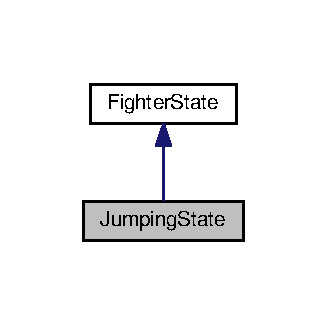
\includegraphics[width=157pt]{classJumpingState__inherit__graph}
\end{center}
\end{figure}


Collaboration diagram for Jumping\+State\+:
\nopagebreak
\begin{figure}[H]
\begin{center}
\leavevmode
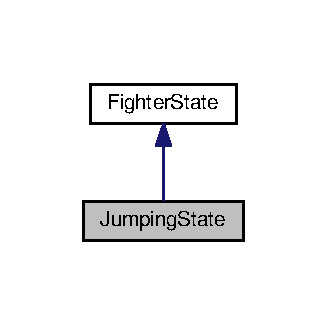
\includegraphics[width=157pt]{classJumpingState__coll__graph}
\end{center}
\end{figure}
\subsection*{Public Member Functions}
\begin{DoxyCompactItemize}
\item 
\hyperlink{classJumpingState_a74a6fbd65de0937c949cb04d7567041f}{Jumping\+State} ()
\item 
virtual void \hyperlink{classJumpingState_a40be6d03f207fc425dfe2b1395fd4edb}{handle\+Input} (\hyperlink{classFighter}{Fighter} \&, \hyperlink{State_8cpp_a080a822f0093973313bd644e517a5090}{Input}) override
\item 
virtual void \hyperlink{classJumpingState_aef36270d1d3aec51bdf4770e9ad571c8}{update} (\hyperlink{classFighter}{Fighter} \&) override
\end{DoxyCompactItemize}
\subsection*{Private Attributes}
\begin{DoxyCompactItemize}
\item 
int \hyperlink{classJumpingState_a89897dfb7cc7758c21b256fc140adc5d}{jumping\+Height}
\end{DoxyCompactItemize}
\subsection*{Additional Inherited Members}


\subsection{Constructor \& Destructor Documentation}
\index{Jumping\+State@{Jumping\+State}!Jumping\+State@{Jumping\+State}}
\index{Jumping\+State@{Jumping\+State}!Jumping\+State@{Jumping\+State}}
\subsubsection[{\texorpdfstring{Jumping\+State()}{JumpingState()}}]{\setlength{\rightskip}{0pt plus 5cm}Jumping\+State\+::\+Jumping\+State (
\begin{DoxyParamCaption}
{}
\end{DoxyParamCaption}
)\hspace{0.3cm}{\ttfamily [inline]}}\hypertarget{classJumpingState_a74a6fbd65de0937c949cb04d7567041f}{}\label{classJumpingState_a74a6fbd65de0937c949cb04d7567041f}

\begin{DoxyCode}
41 \{\hyperlink{classJumpingState_a89897dfb7cc7758c21b256fc140adc5d}{jumpingHeight} = std::rand() % 5 + 1;\}
\end{DoxyCode}


Here is the call graph for this function\+:
\nopagebreak
\begin{figure}[H]
\begin{center}
\leavevmode
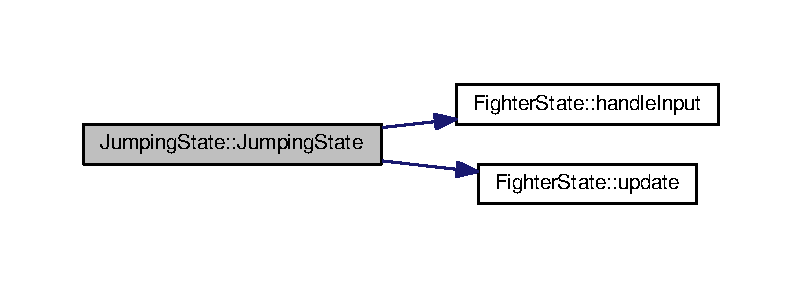
\includegraphics[width=350pt]{classJumpingState_a74a6fbd65de0937c949cb04d7567041f_cgraph}
\end{center}
\end{figure}




\subsection{Member Function Documentation}
\index{Jumping\+State@{Jumping\+State}!handle\+Input@{handle\+Input}}
\index{handle\+Input@{handle\+Input}!Jumping\+State@{Jumping\+State}}
\subsubsection[{\texorpdfstring{handle\+Input(\+Fighter \&, Input) override}{handleInput(Fighter &, Input) override}}]{\setlength{\rightskip}{0pt plus 5cm}void Jumping\+State\+::handle\+Input (
\begin{DoxyParamCaption}
\item[{{\bf Fighter} \&}]{fighter, }
\item[{{\bf Input}}]{input}
\end{DoxyParamCaption}
)\hspace{0.3cm}{\ttfamily [override]}, {\ttfamily [virtual]}}\hypertarget{classJumpingState_a40be6d03f207fc425dfe2b1395fd4edb}{}\label{classJumpingState_a40be6d03f207fc425dfe2b1395fd4edb}


Implements \hyperlink{classFighterState_a84fcd7da4d232e79e1be9b32c0767861}{Fighter\+State}.


\begin{DoxyCode}
113                                                               \{
114     \textcolor{keywordflow}{switch} (input) \{
115         \textcolor{keywordflow}{case} \hyperlink{State_8cpp_a080a822f0093973313bd644e517a5090a6e996a016e50356853001a7c431fa255}{DIVE}:  fighter.\hyperlink{classFighter_add08055f60abd6e9235291b653f65be5}{changeState} (\hyperlink{classFighterState_ad4f8371e5a2d9e5b165d5c41072eb6d9}{FighterState::diving});  \textcolor{keywordflow}{return} 
      fighter.\hyperlink{classFighter_a56cef6bffcdf9775f9d924cd213ed704}{dives}();
116         \textcolor{keywordflow}{default}:
117             std::cout << \textcolor{stringliteral}{"One cannot do that in the middle of a jump.  "} << fighter.
      \hyperlink{classFighter_aea4a9cf98a672b2305d1147885b91c34}{getName}() << \textcolor{stringliteral}{" lands from his jump and is now standing again."} << std::endl;
118             fighter.\hyperlink{classFighter_add08055f60abd6e9235291b653f65be5}{changeState} (\hyperlink{classFighterState_a050e9b5aff81843be5feea296a586889}{FighterState::standing});
119     \}
120 \}
\end{DoxyCode}


Here is the call graph for this function\+:
\nopagebreak
\begin{figure}[H]
\begin{center}
\leavevmode
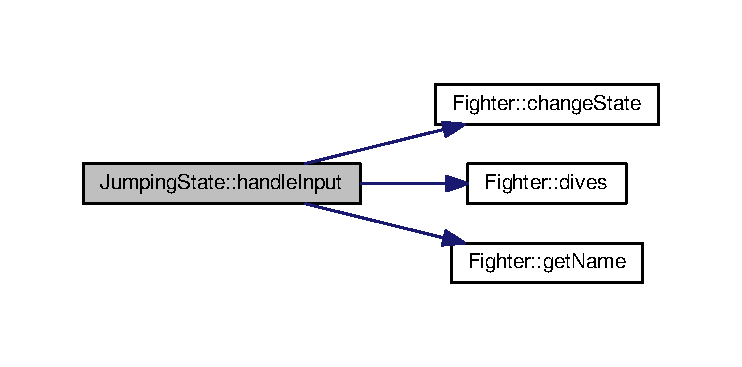
\includegraphics[width=350pt]{classJumpingState_a40be6d03f207fc425dfe2b1395fd4edb_cgraph}
\end{center}
\end{figure}


\index{Jumping\+State@{Jumping\+State}!update@{update}}
\index{update@{update}!Jumping\+State@{Jumping\+State}}
\subsubsection[{\texorpdfstring{update(\+Fighter \&) override}{update(Fighter &) override}}]{\setlength{\rightskip}{0pt plus 5cm}void Jumping\+State\+::update (
\begin{DoxyParamCaption}
\item[{{\bf Fighter} \&}]{fighter}
\end{DoxyParamCaption}
)\hspace{0.3cm}{\ttfamily [override]}, {\ttfamily [virtual]}}\hypertarget{classJumpingState_aef36270d1d3aec51bdf4770e9ad571c8}{}\label{classJumpingState_aef36270d1d3aec51bdf4770e9ad571c8}


Implements \hyperlink{classFighterState_af022f76c6b1fe080047ded2280ec6f8f}{Fighter\+State}.


\begin{DoxyCode}
122                                            \{
123     std::cout << fighter.\hyperlink{classFighter_aea4a9cf98a672b2305d1147885b91c34}{getName}() << \textcolor{stringliteral}{" has jumped "} << \hyperlink{classJumpingState_a89897dfb7cc7758c21b256fc140adc5d}{jumpingHeight} << \textcolor{stringliteral}{" feet into
       the air."} << std::endl;
124     \textcolor{keywordflow}{if} (\hyperlink{classJumpingState_a89897dfb7cc7758c21b256fc140adc5d}{jumpingHeight} >= 3)
125         fighter.\hyperlink{classFighter_aa9c08ec29097e326eab0ffd69db18b9c}{changeFatigueLevelBy}(1);
126 \}
\end{DoxyCode}


Here is the call graph for this function\+:
\nopagebreak
\begin{figure}[H]
\begin{center}
\leavevmode
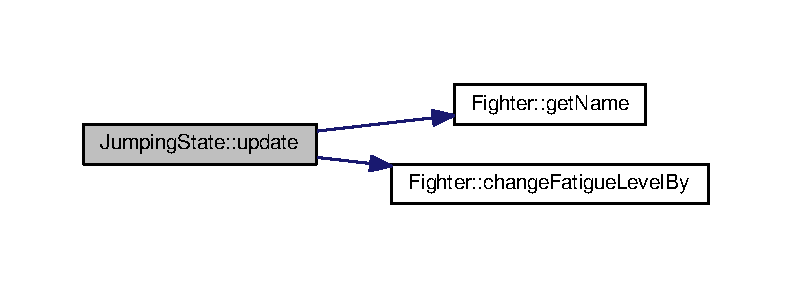
\includegraphics[width=350pt]{classJumpingState_aef36270d1d3aec51bdf4770e9ad571c8_cgraph}
\end{center}
\end{figure}




\subsection{Member Data Documentation}
\index{Jumping\+State@{Jumping\+State}!jumping\+Height@{jumping\+Height}}
\index{jumping\+Height@{jumping\+Height}!Jumping\+State@{Jumping\+State}}
\subsubsection[{\texorpdfstring{jumping\+Height}{jumpingHeight}}]{\setlength{\rightskip}{0pt plus 5cm}int Jumping\+State\+::jumping\+Height\hspace{0.3cm}{\ttfamily [private]}}\hypertarget{classJumpingState_a89897dfb7cc7758c21b256fc140adc5d}{}\label{classJumpingState_a89897dfb7cc7758c21b256fc140adc5d}


The documentation for this class was generated from the following file\+:\begin{DoxyCompactItemize}
\item 
\hyperlink{State_8cpp}{State.\+cpp}\end{DoxyCompactItemize}

\hypertarget{classStandingState}{}\section{Standing\+State Class Reference}
\label{classStandingState}\index{Standing\+State@{Standing\+State}}


Inheritance diagram for Standing\+State\+:
\nopagebreak
\begin{figure}[H]
\begin{center}
\leavevmode
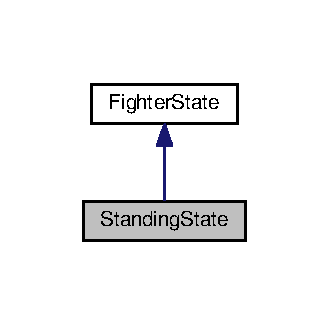
\includegraphics[width=158pt]{classStandingState__inherit__graph}
\end{center}
\end{figure}


Collaboration diagram for Standing\+State\+:
\nopagebreak
\begin{figure}[H]
\begin{center}
\leavevmode
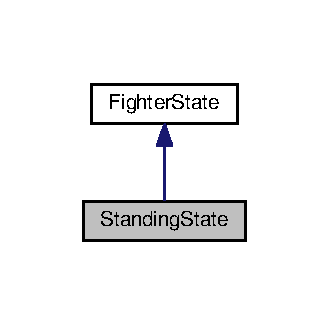
\includegraphics[width=158pt]{classStandingState__coll__graph}
\end{center}
\end{figure}
\subsection*{Public Member Functions}
\begin{DoxyCompactItemize}
\item 
virtual void \hyperlink{classStandingState_a63e99bb4fb71ef88ba573ad902337e7c}{handle\+Input} (\hyperlink{classFighter}{Fighter} \&, \hyperlink{State_8cpp_a080a822f0093973313bd644e517a5090}{Input}) override
\item 
virtual void \hyperlink{classStandingState_a3a99901a53764049b39df5b8f016fb66}{update} (\hyperlink{classFighter}{Fighter} \&) override
\end{DoxyCompactItemize}
\subsection*{Additional Inherited Members}


\subsection{Member Function Documentation}
\index{Standing\+State@{Standing\+State}!handle\+Input@{handle\+Input}}
\index{handle\+Input@{handle\+Input}!Standing\+State@{Standing\+State}}
\subsubsection[{\texorpdfstring{handle\+Input(\+Fighter \&, Input) override}{handleInput(Fighter &, Input) override}}]{\setlength{\rightskip}{0pt plus 5cm}void Standing\+State\+::handle\+Input (
\begin{DoxyParamCaption}
\item[{{\bf Fighter} \&}]{fighter, }
\item[{{\bf Input}}]{input}
\end{DoxyParamCaption}
)\hspace{0.3cm}{\ttfamily [override]}, {\ttfamily [virtual]}}\hypertarget{classStandingState_a63e99bb4fb71ef88ba573ad902337e7c}{}\label{classStandingState_a63e99bb4fb71ef88ba573ad902337e7c}


Implements \hyperlink{classFighterState_a84fcd7da4d232e79e1be9b32c0767861}{Fighter\+State}.


\begin{DoxyCode}
76                                                                \{
77     \textcolor{keywordflow}{switch} (input) \{
78         \textcolor{keywordflow}{case} \hyperlink{State_8cpp_a080a822f0093973313bd644e517a5090a4e0f05b608ae82cd3d38087399f6962a}{STAND\_UP}:  std::cout << fighter.\hyperlink{classFighter_aea4a9cf98a672b2305d1147885b91c34}{getName}() << \textcolor{stringliteral}{" remains standing."} << std::endl;
        \textcolor{keywordflow}{return};
79         \textcolor{keywordflow}{case} \hyperlink{State_8cpp_a080a822f0093973313bd644e517a5090af82233b8404f602e50c8fb3fff20db8d}{DUCK\_DOWN}:  fighter.\hyperlink{classFighter_add08055f60abd6e9235291b653f65be5}{changeState} (std::shared\_ptr<DuckingState> (\textcolor{keyword}{new} 
      \hyperlink{classDuckingState}{DuckingState}));  \textcolor{keywordflow}{return} fighter.\hyperlink{classFighter_afff11a1b3dacee662cb3fbe35f54df17}{ducksDown}();
80         \textcolor{keywordflow}{case} \hyperlink{State_8cpp_a080a822f0093973313bd644e517a5090a1f28d4392b1c1e7da2af2283632d81e1}{JUMP}:  fighter.\hyperlink{classFighter_a32a4250077afba9b3629a8f553dd8776}{jumps}();  \textcolor{keywordflow}{return} fighter.\hyperlink{classFighter_add08055f60abd6e9235291b653f65be5}{changeState} (
      std::shared\_ptr<JumpingState> (\textcolor{keyword}{new} \hyperlink{classJumpingState}{JumpingState}));
81         \textcolor{keywordflow}{default}:  std::cout << \textcolor{stringliteral}{"One cannot do that while standing.  "} << fighter.
      \hyperlink{classFighter_aea4a9cf98a672b2305d1147885b91c34}{getName}() << \textcolor{stringliteral}{" remains standing by default."} << std::endl;
82     \}
83 \}
\end{DoxyCode}


Here is the call graph for this function\+:
\nopagebreak
\begin{figure}[H]
\begin{center}
\leavevmode
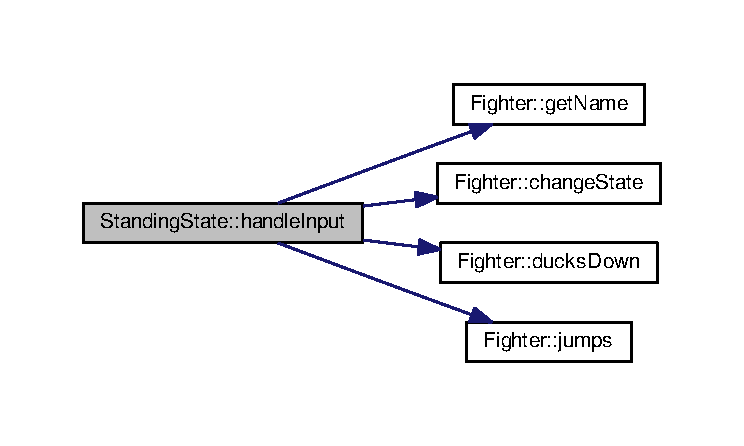
\includegraphics[width=350pt]{classStandingState_a63e99bb4fb71ef88ba573ad902337e7c_cgraph}
\end{center}
\end{figure}


\index{Standing\+State@{Standing\+State}!update@{update}}
\index{update@{update}!Standing\+State@{Standing\+State}}
\subsubsection[{\texorpdfstring{update(\+Fighter \&) override}{update(Fighter &) override}}]{\setlength{\rightskip}{0pt plus 5cm}void Standing\+State\+::update (
\begin{DoxyParamCaption}
\item[{{\bf Fighter} \&}]{fighter}
\end{DoxyParamCaption}
)\hspace{0.3cm}{\ttfamily [override]}, {\ttfamily [virtual]}}\hypertarget{classStandingState_a3a99901a53764049b39df5b8f016fb66}{}\label{classStandingState_a3a99901a53764049b39df5b8f016fb66}


Implements \hyperlink{classFighterState_af022f76c6b1fe080047ded2280ec6f8f}{Fighter\+State}.


\begin{DoxyCode}
85                                             \{
86     \textcolor{keywordflow}{if} (fighter.\hyperlink{classFighter_a1bc4025d988b66dfceaf0005e74f34ff}{getFatigueLevel}() > 0)
87         fighter.\hyperlink{classFighter_aa9c08ec29097e326eab0ffd69db18b9c}{changeFatigueLevelBy}(-1);
88 \}
\end{DoxyCode}


Here is the call graph for this function\+:
\nopagebreak
\begin{figure}[H]
\begin{center}
\leavevmode
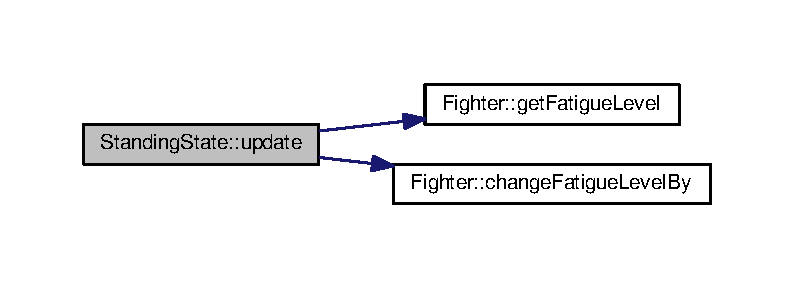
\includegraphics[width=350pt]{classStandingState_a3a99901a53764049b39df5b8f016fb66_cgraph}
\end{center}
\end{figure}




The documentation for this class was generated from the following file\+:\begin{DoxyCompactItemize}
\item 
\hyperlink{State_8cpp}{State.\+cpp}\end{DoxyCompactItemize}

\chapter{File Documentation}
\hypertarget{State_8cpp}{}\section{State.\+cpp File Reference}
\label{State_8cpp}\index{State.\+cpp@{State.\+cpp}}
{\ttfamily \#include $<$iostream$>$}\\*
{\ttfamily \#include $<$string$>$}\\*
{\ttfamily \#include $<$cstdlib$>$}\\*
{\ttfamily \#include $<$ctime$>$}\\*
{\ttfamily \#include $<$memory$>$}\\*
Include dependency graph for State.\+cpp\+:
\nopagebreak
\begin{figure}[H]
\begin{center}
\leavevmode
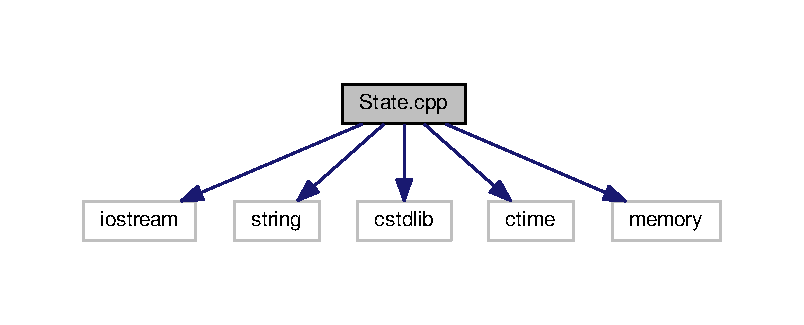
\includegraphics[width=350pt]{State_8cpp__incl}
\end{center}
\end{figure}
\subsection*{Classes}
\begin{DoxyCompactItemize}
\item 
class \hyperlink{classFighterState}{Fighter\+State}
\item 
class \hyperlink{classDuckingState}{Ducking\+State}
\item 
class \hyperlink{classStandingState}{Standing\+State}
\item 
class \hyperlink{classJumpingState}{Jumping\+State}
\item 
class \hyperlink{classDivingState}{Diving\+State}
\item 
class \hyperlink{classFighter}{Fighter}
\end{DoxyCompactItemize}
\subsection*{Enumerations}
\begin{DoxyCompactItemize}
\item 
enum \hyperlink{State_8cpp_a080a822f0093973313bd644e517a5090}{Input} \{ \hyperlink{State_8cpp_a080a822f0093973313bd644e517a5090af82233b8404f602e50c8fb3fff20db8d}{D\+U\+C\+K\+\_\+\+D\+O\+WN}, 
\hyperlink{State_8cpp_a080a822f0093973313bd644e517a5090a4e0f05b608ae82cd3d38087399f6962a}{S\+T\+A\+N\+D\+\_\+\+UP}, 
\hyperlink{State_8cpp_a080a822f0093973313bd644e517a5090a1f28d4392b1c1e7da2af2283632d81e1}{J\+U\+MP}, 
\hyperlink{State_8cpp_a080a822f0093973313bd644e517a5090a6e996a016e50356853001a7c431fa255}{D\+I\+VE}
 \}
\end{DoxyCompactItemize}
\subsection*{Functions}
\begin{DoxyCompactItemize}
\item 
int \hyperlink{State_8cpp_ae66f6b31b5ad750f1fe042a706a4e3d4}{main} ()
\end{DoxyCompactItemize}


\subsection{Enumeration Type Documentation}
\index{State.\+cpp@{State.\+cpp}!Input@{Input}}
\index{Input@{Input}!State.\+cpp@{State.\+cpp}}
\subsubsection[{\texorpdfstring{Input}{Input}}]{\setlength{\rightskip}{0pt plus 5cm}enum {\bf Input}}\hypertarget{State_8cpp_a080a822f0093973313bd644e517a5090}{}\label{State_8cpp_a080a822f0093973313bd644e517a5090}
\begin{Desc}
\item[Enumerator]\par
\begin{description}
\index{D\+U\+C\+K\+\_\+\+D\+O\+WN@{D\+U\+C\+K\+\_\+\+D\+O\+WN}!State.\+cpp@{State.\+cpp}}\index{State.\+cpp@{State.\+cpp}!D\+U\+C\+K\+\_\+\+D\+O\+WN@{D\+U\+C\+K\+\_\+\+D\+O\+WN}}\item[{\em 
D\+U\+C\+K\+\_\+\+D\+O\+WN\hypertarget{State_8cpp_a080a822f0093973313bd644e517a5090af82233b8404f602e50c8fb3fff20db8d}{}\label{State_8cpp_a080a822f0093973313bd644e517a5090af82233b8404f602e50c8fb3fff20db8d}
}]\index{S\+T\+A\+N\+D\+\_\+\+UP@{S\+T\+A\+N\+D\+\_\+\+UP}!State.\+cpp@{State.\+cpp}}\index{State.\+cpp@{State.\+cpp}!S\+T\+A\+N\+D\+\_\+\+UP@{S\+T\+A\+N\+D\+\_\+\+UP}}\item[{\em 
S\+T\+A\+N\+D\+\_\+\+UP\hypertarget{State_8cpp_a080a822f0093973313bd644e517a5090a4e0f05b608ae82cd3d38087399f6962a}{}\label{State_8cpp_a080a822f0093973313bd644e517a5090a4e0f05b608ae82cd3d38087399f6962a}
}]\index{J\+U\+MP@{J\+U\+MP}!State.\+cpp@{State.\+cpp}}\index{State.\+cpp@{State.\+cpp}!J\+U\+MP@{J\+U\+MP}}\item[{\em 
J\+U\+MP\hypertarget{State_8cpp_a080a822f0093973313bd644e517a5090a1f28d4392b1c1e7da2af2283632d81e1}{}\label{State_8cpp_a080a822f0093973313bd644e517a5090a1f28d4392b1c1e7da2af2283632d81e1}
}]\index{D\+I\+VE@{D\+I\+VE}!State.\+cpp@{State.\+cpp}}\index{State.\+cpp@{State.\+cpp}!D\+I\+VE@{D\+I\+VE}}\item[{\em 
D\+I\+VE\hypertarget{State_8cpp_a080a822f0093973313bd644e517a5090a6e996a016e50356853001a7c431fa255}{}\label{State_8cpp_a080a822f0093973313bd644e517a5090a6e996a016e50356853001a7c431fa255}
}]\end{description}
\end{Desc}

\begin{DoxyCode}
7 \{\hyperlink{State_8cpp_a080a822f0093973313bd644e517a5090af82233b8404f602e50c8fb3fff20db8d}{DUCK\_DOWN}, \hyperlink{State_8cpp_a080a822f0093973313bd644e517a5090a4e0f05b608ae82cd3d38087399f6962a}{STAND\_UP}, \hyperlink{State_8cpp_a080a822f0093973313bd644e517a5090a1f28d4392b1c1e7da2af2283632d81e1}{JUMP}, \hyperlink{State_8cpp_a080a822f0093973313bd644e517a5090a6e996a016e50356853001a7c431fa255}{DIVE}\};
\end{DoxyCode}


\subsection{Function Documentation}
\index{State.\+cpp@{State.\+cpp}!main@{main}}
\index{main@{main}!State.\+cpp@{State.\+cpp}}
\subsubsection[{\texorpdfstring{main()}{main()}}]{\setlength{\rightskip}{0pt plus 5cm}int main (
\begin{DoxyParamCaption}
{}
\end{DoxyParamCaption}
)}\hypertarget{State_8cpp_ae66f6b31b5ad750f1fe042a706a4e3d4}{}\label{State_8cpp_ae66f6b31b5ad750f1fe042a706a4e3d4}

\begin{DoxyCode}
137            \{
138     std::srand(std::time(\textcolor{keyword}{nullptr}));
139     \hyperlink{classFighter}{Fighter} rex (\textcolor{stringliteral}{"Rex the Fighter"}), borg (\textcolor{stringliteral}{"Borg the Fighter"});
140     std::cout << rex.getName() << \textcolor{stringliteral}{" and "} << borg.getName() << \textcolor{stringliteral}{" are currently standing."} << std::endl;
141     \textcolor{keywordtype}{int} choice;
142     \textcolor{keyword}{auto} chooseAction = [&choice](\hyperlink{classFighter}{Fighter}& fighter) \{
143         std::cout << std::endl << \hyperlink{State_8cpp_a080a822f0093973313bd644e517a5090af82233b8404f602e50c8fb3fff20db8d}{DUCK\_DOWN} + 1 << \textcolor{stringliteral}{") Duck down  "} << 
      \hyperlink{State_8cpp_a080a822f0093973313bd644e517a5090a4e0f05b608ae82cd3d38087399f6962a}{STAND\_UP} + 1 << \textcolor{stringliteral}{") Stand up  "} << \hyperlink{State_8cpp_a080a822f0093973313bd644e517a5090a1f28d4392b1c1e7da2af2283632d81e1}{JUMP} + 1
144             << \textcolor{stringliteral}{") Jump  "} << \hyperlink{State_8cpp_a080a822f0093973313bd644e517a5090a6e996a016e50356853001a7c431fa255}{DIVE} + 1 << \textcolor{stringliteral}{") Dive in the middle of a jump"} << std::endl;
145         std::cout << \textcolor{stringliteral}{"Choice for "} << fighter.getName() << \textcolor{stringliteral}{"? "};
146         std::cin >> choice;
147         \textcolor{keyword}{const} \hyperlink{State_8cpp_a080a822f0093973313bd644e517a5090}{Input} input1 = \textcolor{keyword}{static\_cast<}\hyperlink{State_8cpp_a080a822f0093973313bd644e517a5090}{Input}\textcolor{keyword}{>}(choice - 1);
148         fighter.handleInput (input1);   
149     \};
150     \textcolor{keywordflow}{while} (\textcolor{keyword}{true}) \{
151         chooseAction (rex);
152         chooseAction (borg);
153     \}
154 \}\end{DoxyCode}


Here is the call graph for this function\+:
\nopagebreak
\begin{figure}[H]
\begin{center}
\leavevmode
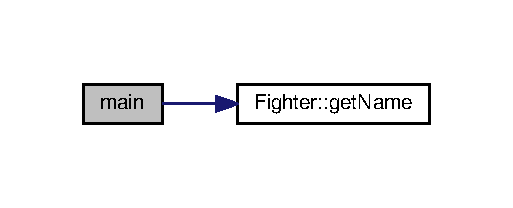
\includegraphics[width=246pt]{State_8cpp_ae66f6b31b5ad750f1fe042a706a4e3d4_cgraph}
\end{center}
\end{figure}



%--- End generated contents ---

% Index
\backmatter
\newpage
\phantomsection
\clearemptydoublepage
\addcontentsline{toc}{chapter}{Index}
\printindex

\end{document}
